{\bf BME154L - Spring 2012 - Exam \#2 Solutions}\hfill Name (Net ID):\underline{\hspace*{3.0in}}



\section{[25 points]}

\begin{tabular}{cc}
\centering
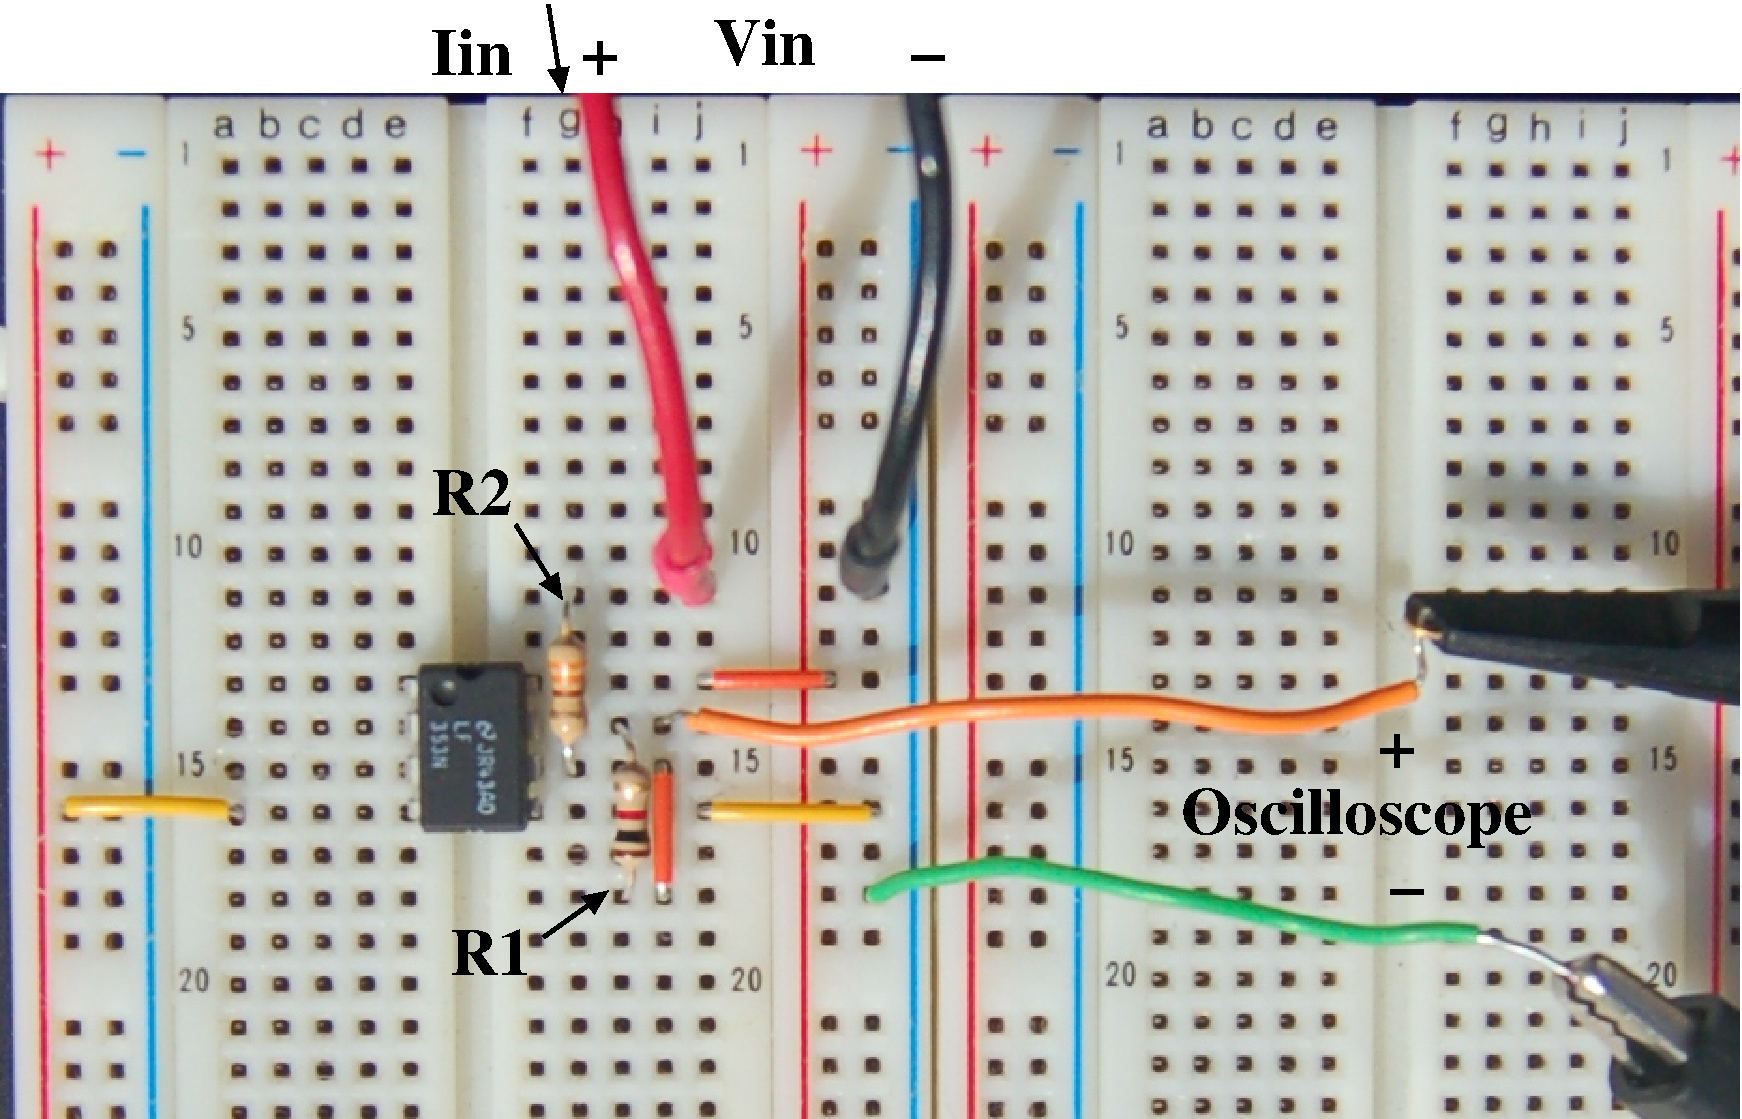
\includegraphics[width=0.6\linewidth]{breadboard_ckt_labeled} &
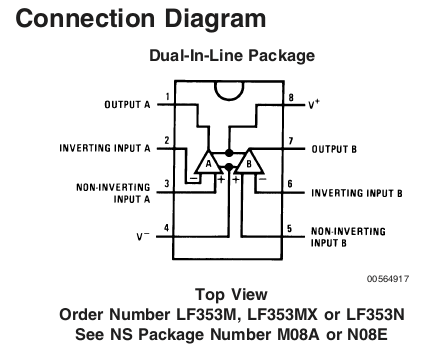
\includegraphics[width=0.4\linewidth]{LF353_Connection_Diagram} \\
\end{tabular}

You have built the circuit above in lab using the chip with the included relevant pin diagram, where $R_1$ = 20 k$\Omega$ and $R_2$ = 10 k$\Omega$.  

\begin{enumerate}
\item Draw the circuit schematic associated with this photograph, labeling $R_1$ and $R_2$, GND, and the connections for $V_{in}$ and the oscilloscope.
\item Briefly describe how you would go about measuring the input current into
this circuit ($i_{in}$) using the procedures you commonly use in lab.
\item The power supply has not been attached to this breadboard.  Clearly
indicate where you would make those connections on the breadboard diagram (-12
V, GND, +12 V).
\item Your lab partner mistakenly pulls $R_1$ completely out of your
breadboard, but everything else is intact.  Sketch the transfer functions of
this circuit for $V_{in}$ = [-1.5:1.5] V \underline{with} and
\underline{without} $R_1$ in the breadboard on the same plot.
\end{enumerate}

\clearpage

{\bf BME154L - Spring 2012 - Exam \#2 Solutions}\hfill Name (Net ID):\underline{\hspace*{3.0in}}



\clearpage
